% Title: Report LaTex File: Hardware Development
% Auther: DC Eksteen
% Student Number: 22623906
% Contact: 22623906@sun.ac.za
% Date: 2022/09/14
% Version: 2.0

\chapter{Hardware Development}
% Section overview: Hardware development.

For the project, hardware was developed with the aim of achieving the objectives shown in \ref{tab:devgoals} below:

\begin{table}[H]
	\renewcommand{\arraystretch}{\tablestretch}
	\centering
	\caption{Objectives of Hardware Development}
	\begin{tabularx}{\textwidth}{p{3.2cm} >{\raggedright}X >{\raggedright\arraybackslash}p{2cm}}
		\toprule
		      & Description & Reference \\
		\midrule
		HDO 1 &             & ER x      \\
		HDO 2 &             & ER x      \\
		HDO 3 &             & ER x      \\
		HDO 4 &             & ER x      \\
		\bottomrule
	\end{tabularx}
	\label{tab:devgoals}
\end{table}

\newpage

\section{Roller Design}
\label{sec:opspeed}

Roller trainers require the cyclist to be travelling at some speed for stability. Thus, the expected operating range of a cyclist on the trainer will typically range between \SI{10}{\kilo\meter\per\hour} and \SI{50}{\kilo\meter\per\hour}. For the design, a maximum high speed of \SI{60}{\kilo\meter\per\hour} was considered. The corresponding drum speeds for common drum size options are shown in Figure \ref{fig:speedCalc} below.

\begin{figure}[H]
	\begin{center}
		\includegraphics[width=0.8\textwidth]{SpeedCalculations.jpg}
		\caption{Rotational Speed of Roller Size Comparison}
		\label{fig:speedCalc}
	\end{center}
\end{figure}

Considering the design of the Eddy Current brake, as discussed in Section \ref{sec:Eddy}, higher braking force can be achieved at higher drum speeds, and result in a larger operating range. On the other hand, higher speeds will also increase the free-rolling resistance of the trainer, and allow for less range at higher speeds. Thus, \SI{90}{\milli\meter} drums were identified as a good compromise, and were selected as the best option for the platform.

The rollers were designed to consist of class-12 \acf{upvc} pipes attached to EN-8 steel shafts. The bearings that were used are 6902RS deep groove ball bearings with rubber shields on both sides.

\begin{figure}[H]
	\centering
	\begin{subfigure}{.5\textwidth}
		\centering
		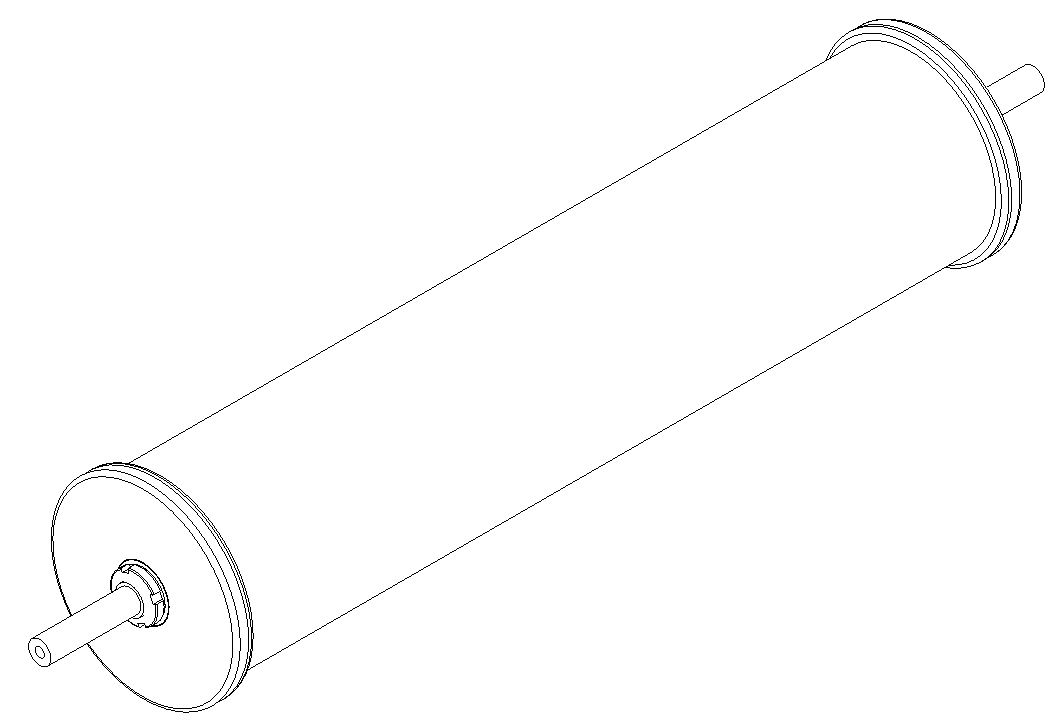
\includegraphics[width=\linewidth]{rollerCad.jpg}
		\caption{Roller Design}
		\label{fig:rollerCAD}
	\end{subfigure}%
	\begin{subfigure}{.5\textwidth}
		\centering
		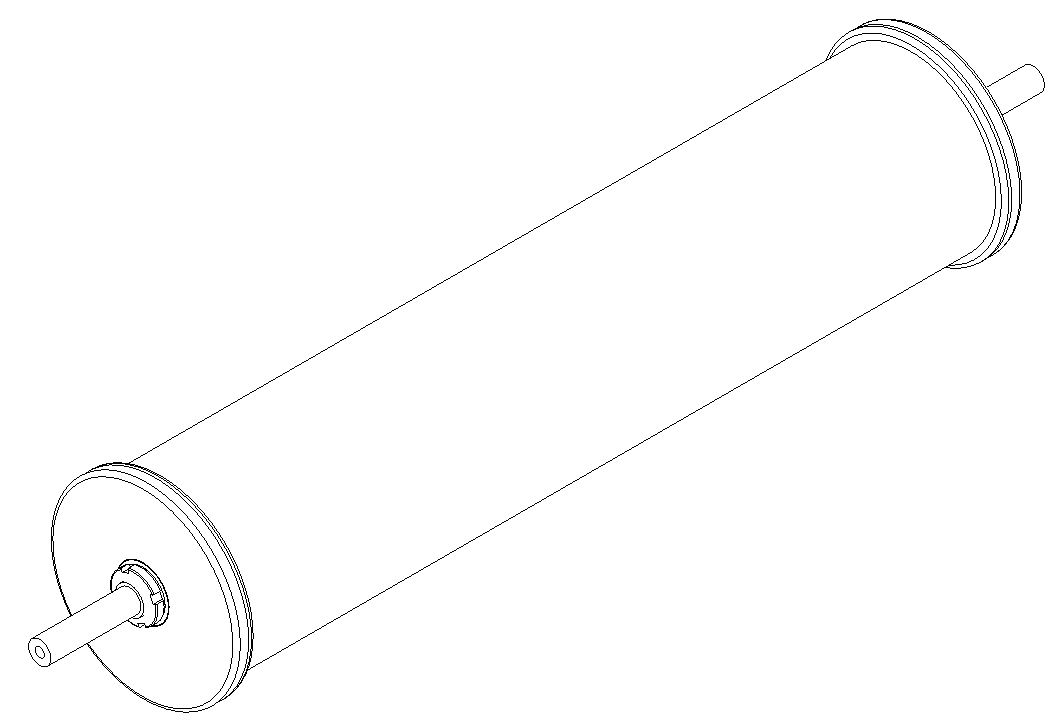
\includegraphics[width=\linewidth]{rollerCad.jpg}
		\caption{Built Roller}
		\label{fig:rollerBuild}
	\end{subfigure}
	\caption{Roller Development}
	\label{fig:rollerDev}
\end{figure}

For the two front idler rollers, the \ac{upvc} pipe and end-caps rotate freely on a a fixed shaft, and are coupled together with a rubber elastic band that is used on existing roller models. The rear roller is attached to the shaft with a key at both end-caps in order to allow for force to be transferred from the braking unit to the rear wheel of the cyclist.

\newpage

\section{Eddy Current Brake Design}
\label{sec:Eddy}

\subsubsection{Braking Torque Requirements}

When considering the \SI{90}{\milli\meter} roller size that was selected in Section \ref{sec:opspeed}, the Torque requirements for different power outputs is shown in Figure \ref{fig:torqueCalc} below. From the figure, it can be seen that the torque requirement at low speeds will dominate the torque requirement and should thus be used as consideration when selecting torque requirements of the brake.

\begin{figure}[H]
	\begin{center}
		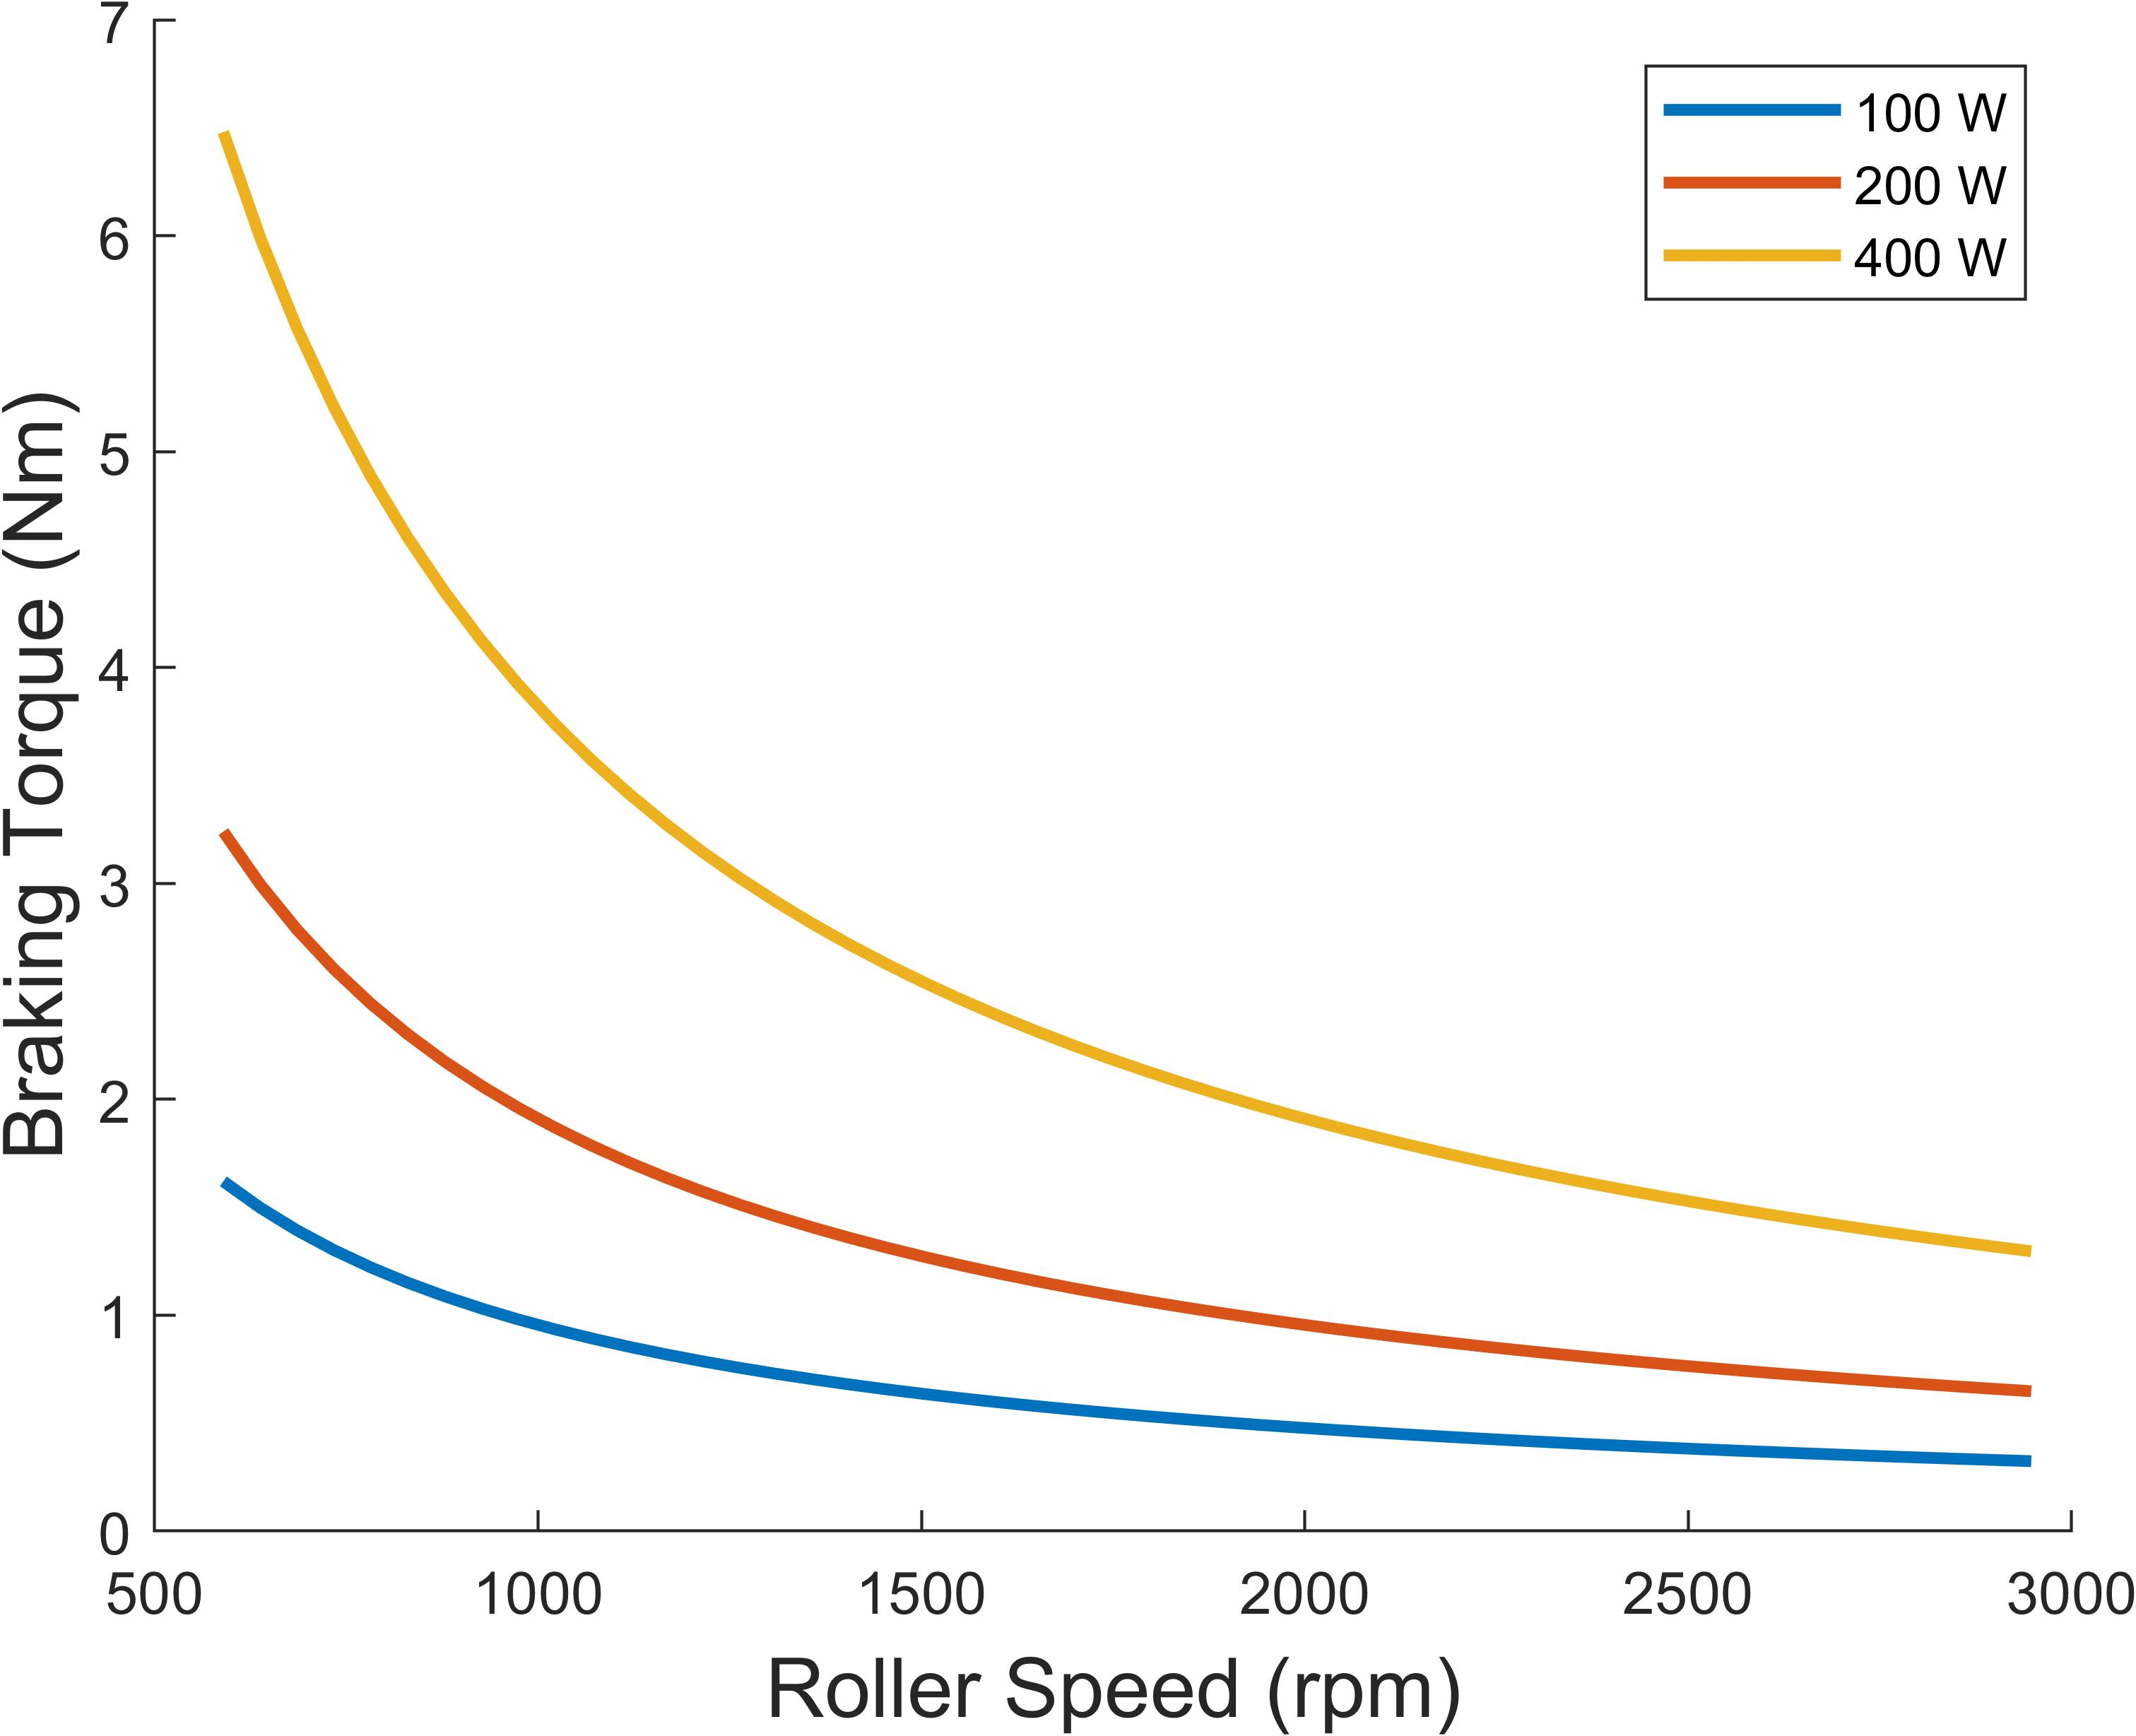
\includegraphics[width=0.8\textwidth]{TorqueCalculations.jpg}
		\caption{Torque Requirement Curve}
		\label{fig:torqueCalc}
	\end{center}
\end{figure}

\subsubsection{Parameter Selection}

For the \ac{ecb}, Neodymium rare earth permanent disk magnets were selected as they would provide the highest magnetic flux density.

\begin{figure}[H]
	\centering
	\begin{subfigure}{.4\textwidth}
		\centering
		\includegraphics[width=0.7\linewidth]{magnetD.jpg}
		\caption{Neodymium Disk Magnet}
		\label{fig:magN}
	\end{subfigure}%
\hfill
	\begin{subfigure}{.4\textwidth}
		\centering
		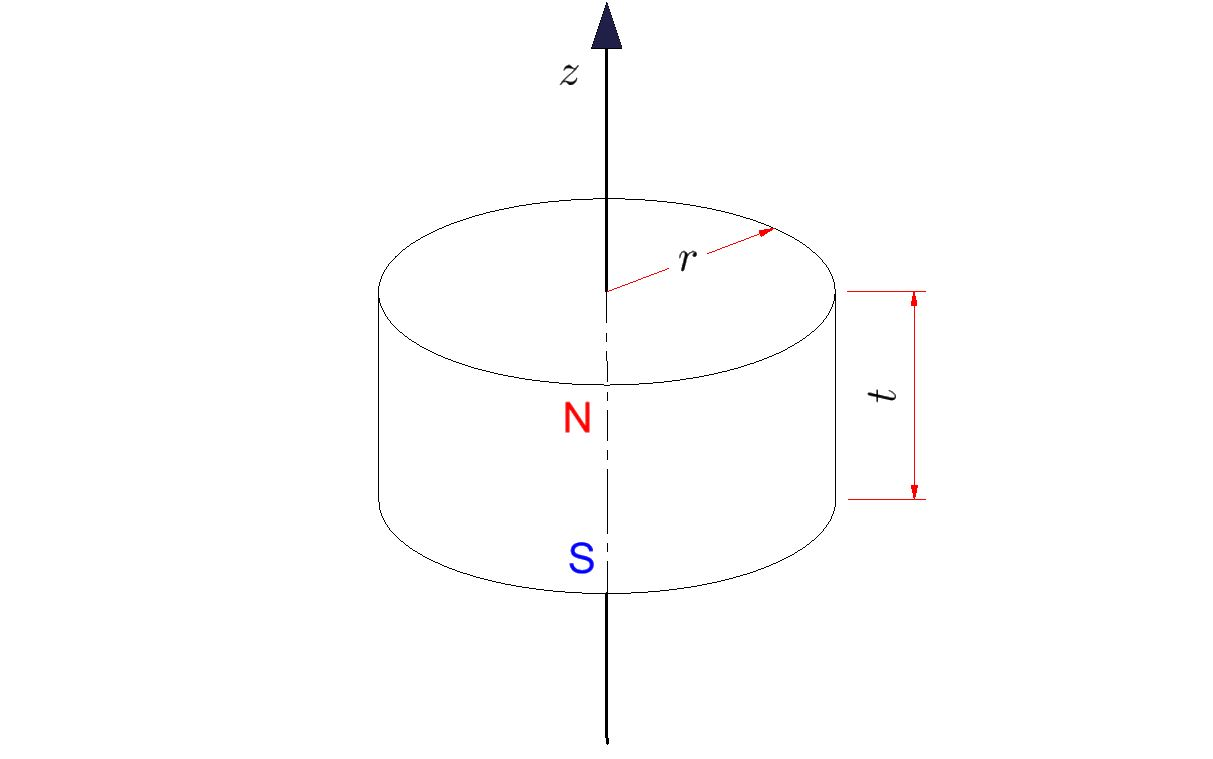
\includegraphics[width=\linewidth]{magnetBr.jpg}
		\caption{\ac{B} Field Calculation}
		\label{fig:B0}
	\end{subfigure}
	\caption{Disk Magnet}
	\citep[Addapted from][]{Supermagnete:2010}
	\label{fig:magnets}
\end{figure}

\begin{equation}
	\acs{B} = \frac{\acs{Br}}{2} (\frac{t+ z}{\sqrt{r^2 + {t + z}^2}} - \frac{z}{r^2 + z^2})
	\label{eq:B}
\end{equation}

\begin{figure}[h!]
	\centering
	\begin{subfigure}[b]{.475\textwidth}
		\centering
		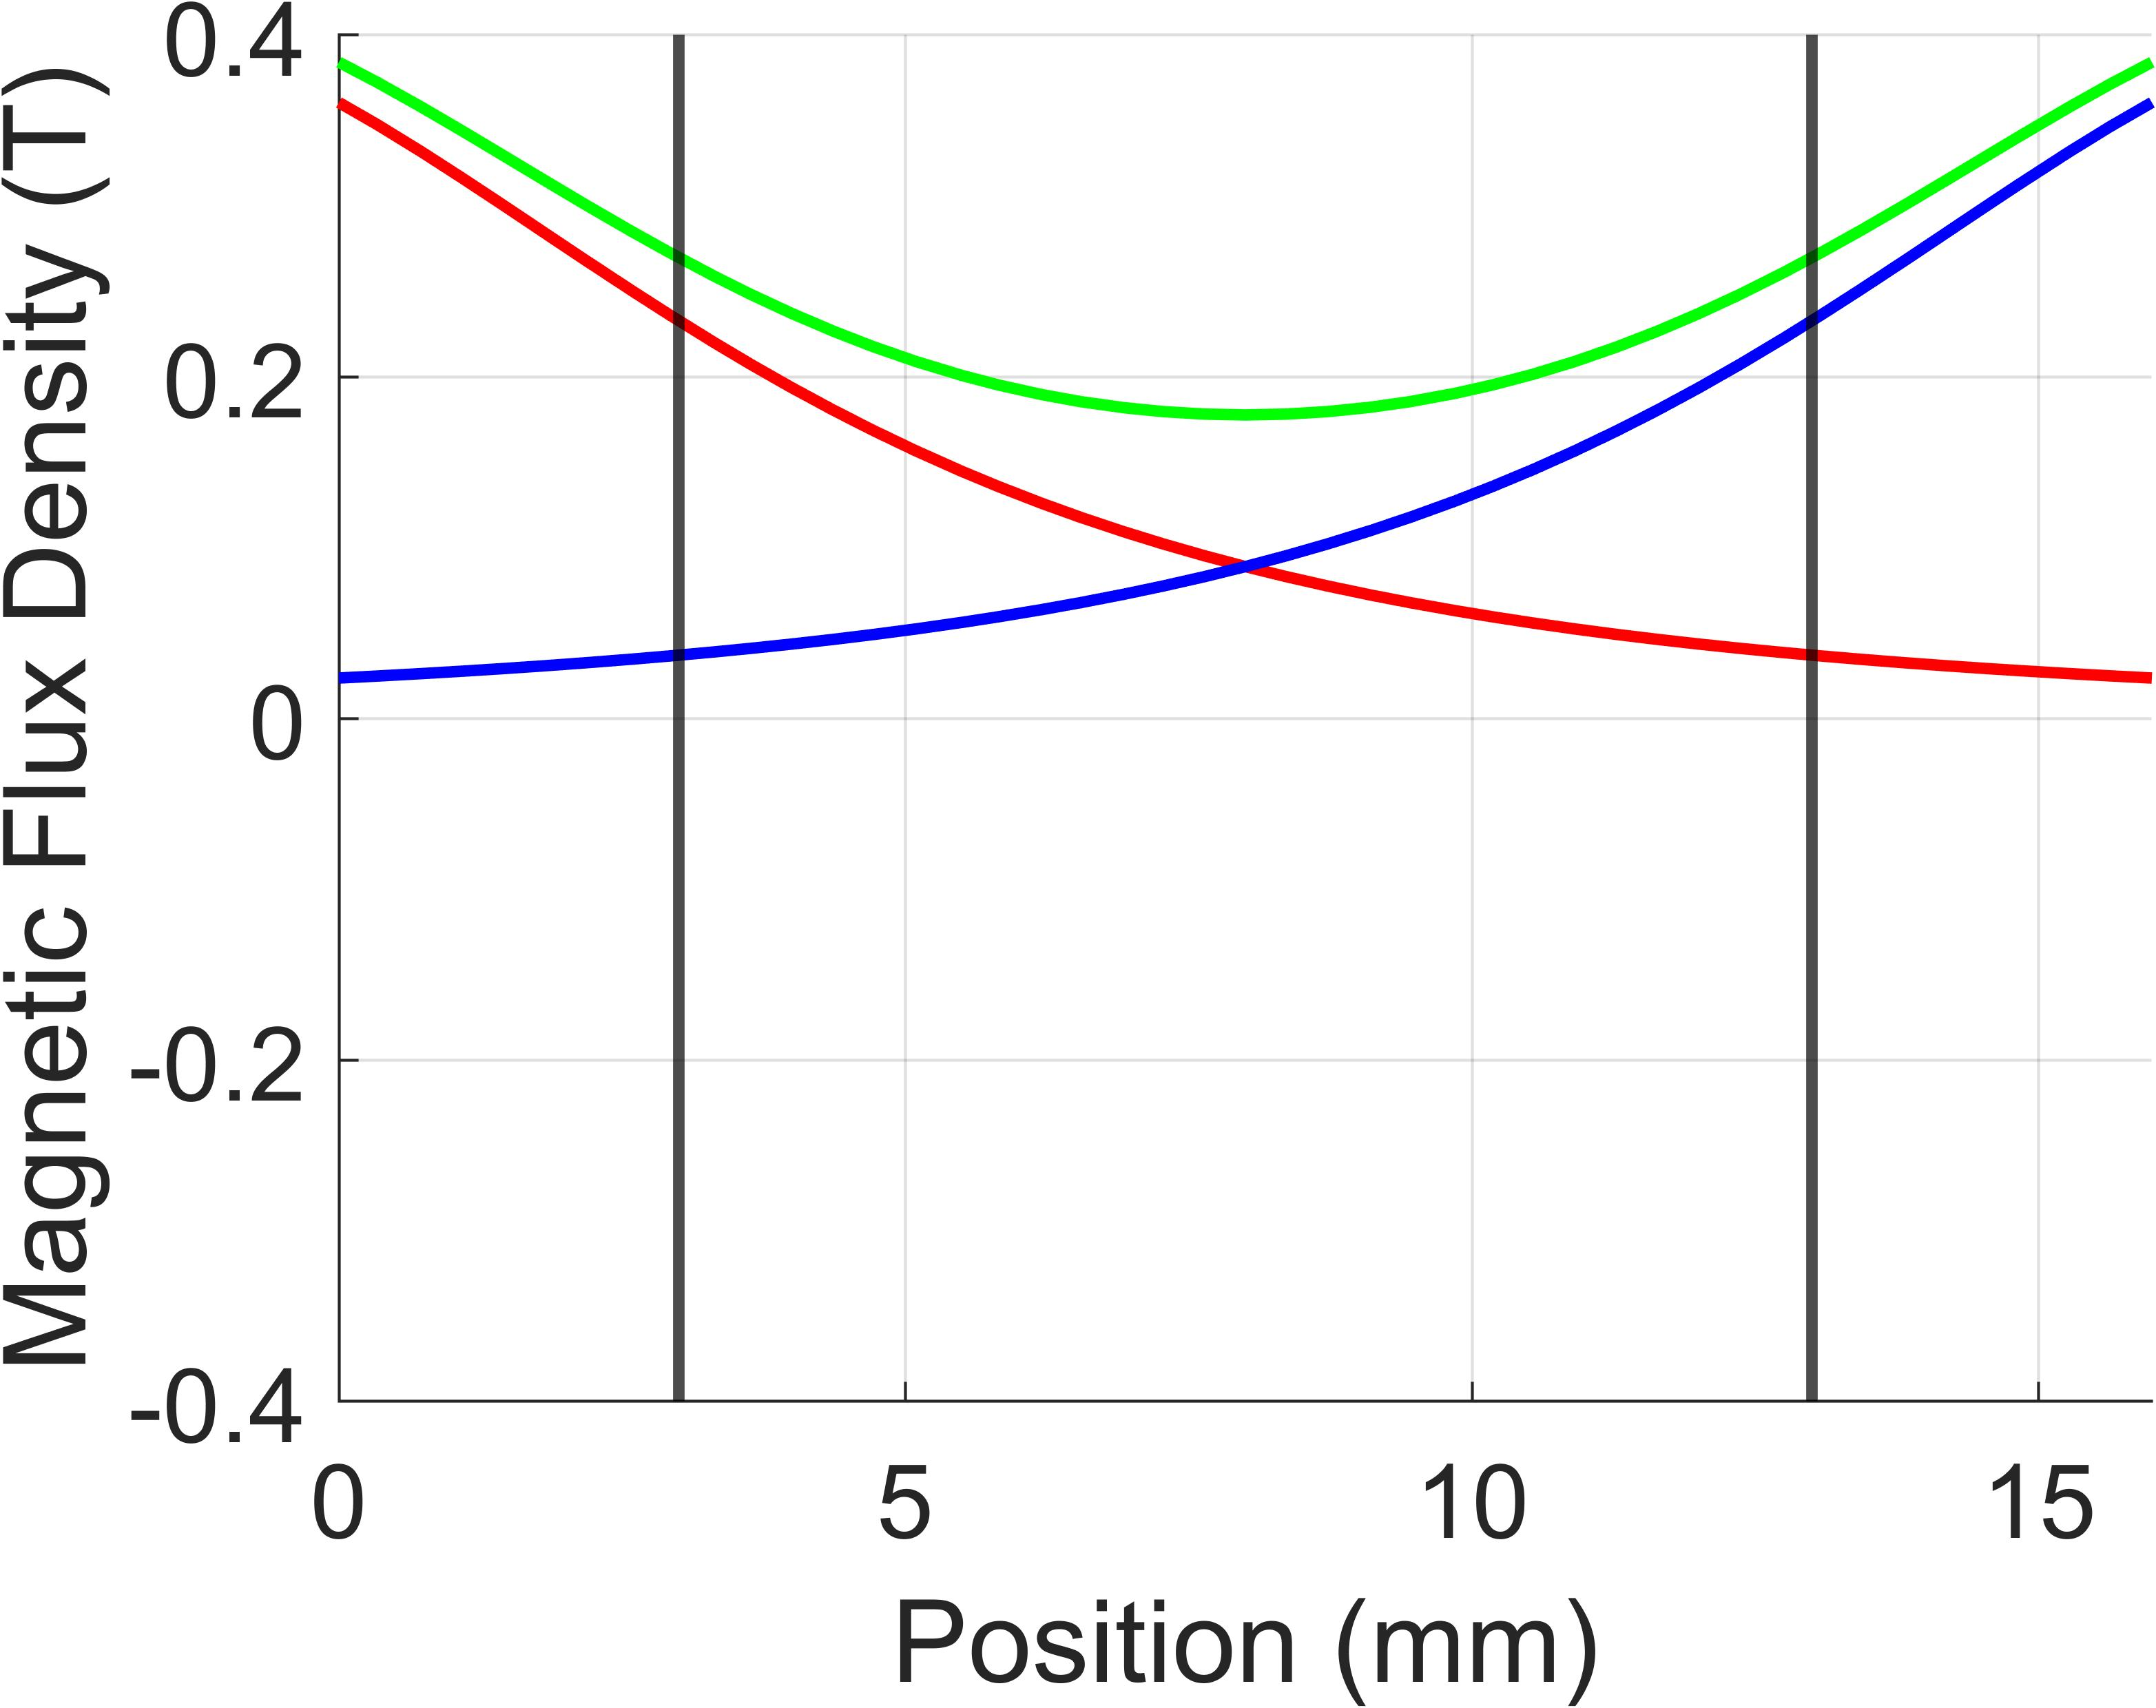
\includegraphics[width=.9\linewidth]{FluxZeroDeg.jpg}
		\caption{\SI{0}{\degree} Phase}
		\label{fig:Flux0}
	\end{subfigure}
	\hfill
	\begin{subfigure}[b]{.475\textwidth}
		\centering
		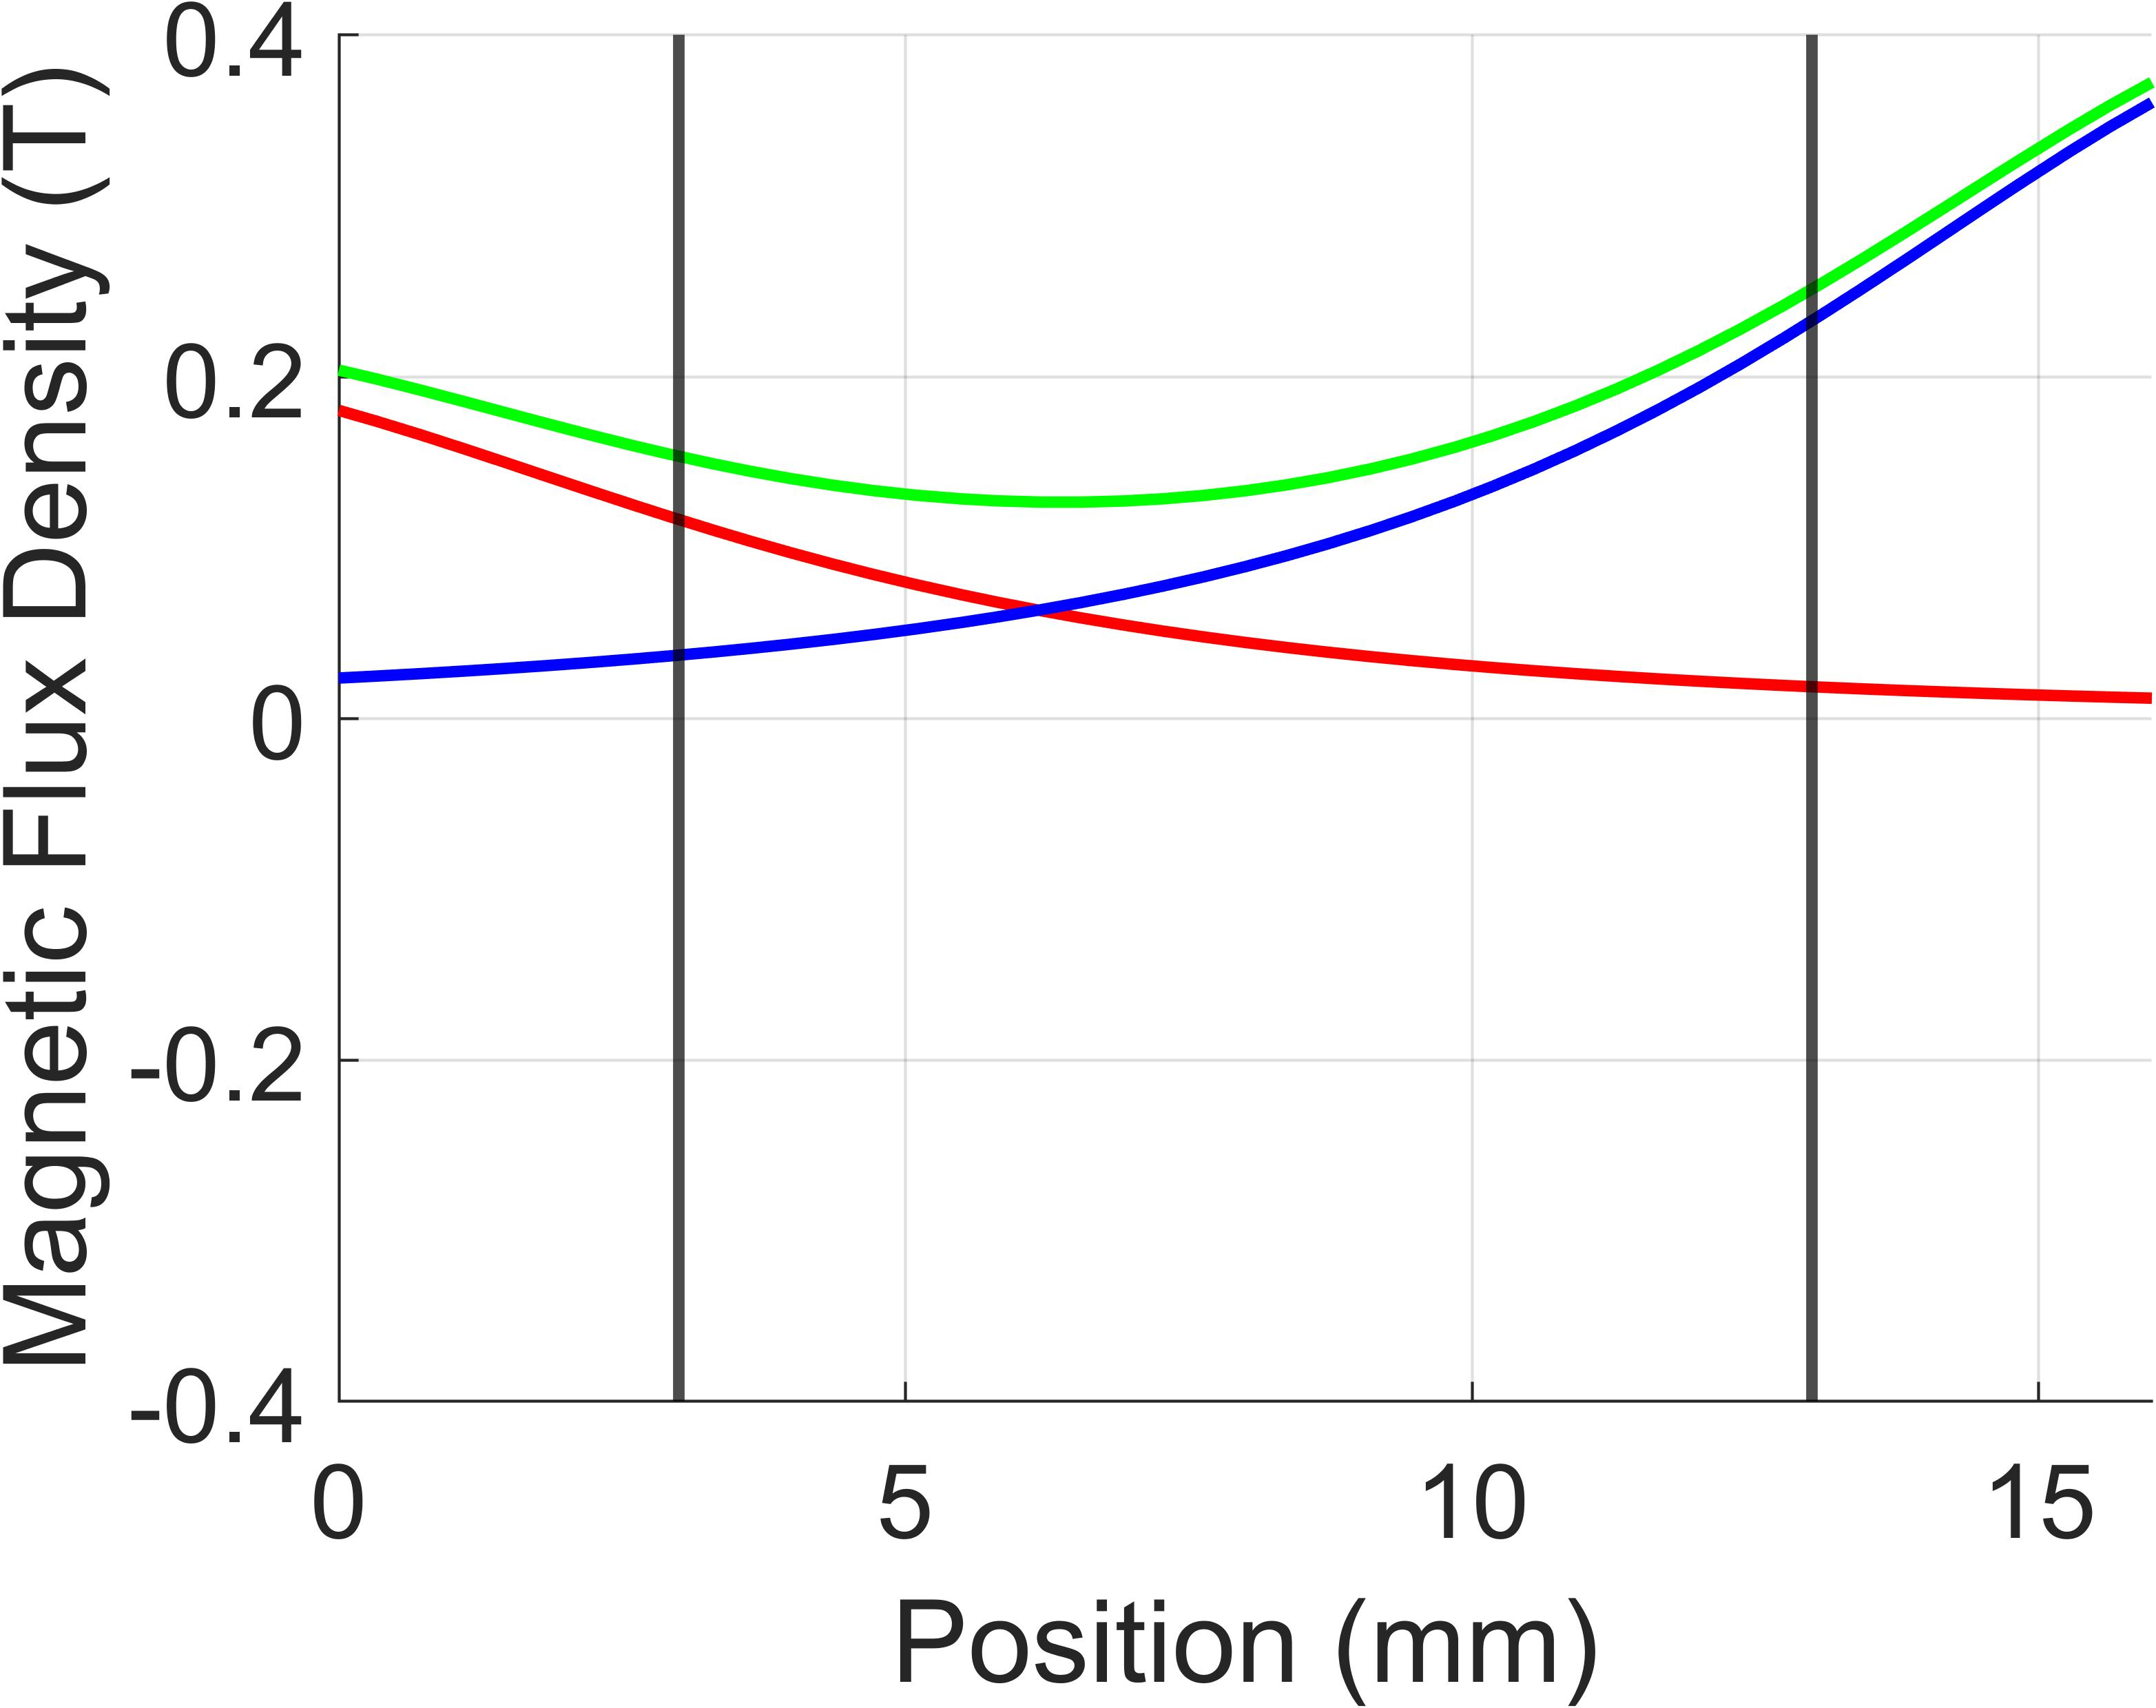
\includegraphics[width=.9\linewidth]{FluxSixtyDeg.jpg}
		\caption{\SI{60}{\degree} Phase}
		\label{fig:Flux60}
	\end{subfigure}
	\vskip\baselineskip
	\begin{subfigure}[b]{.475\textwidth}
		\centering
		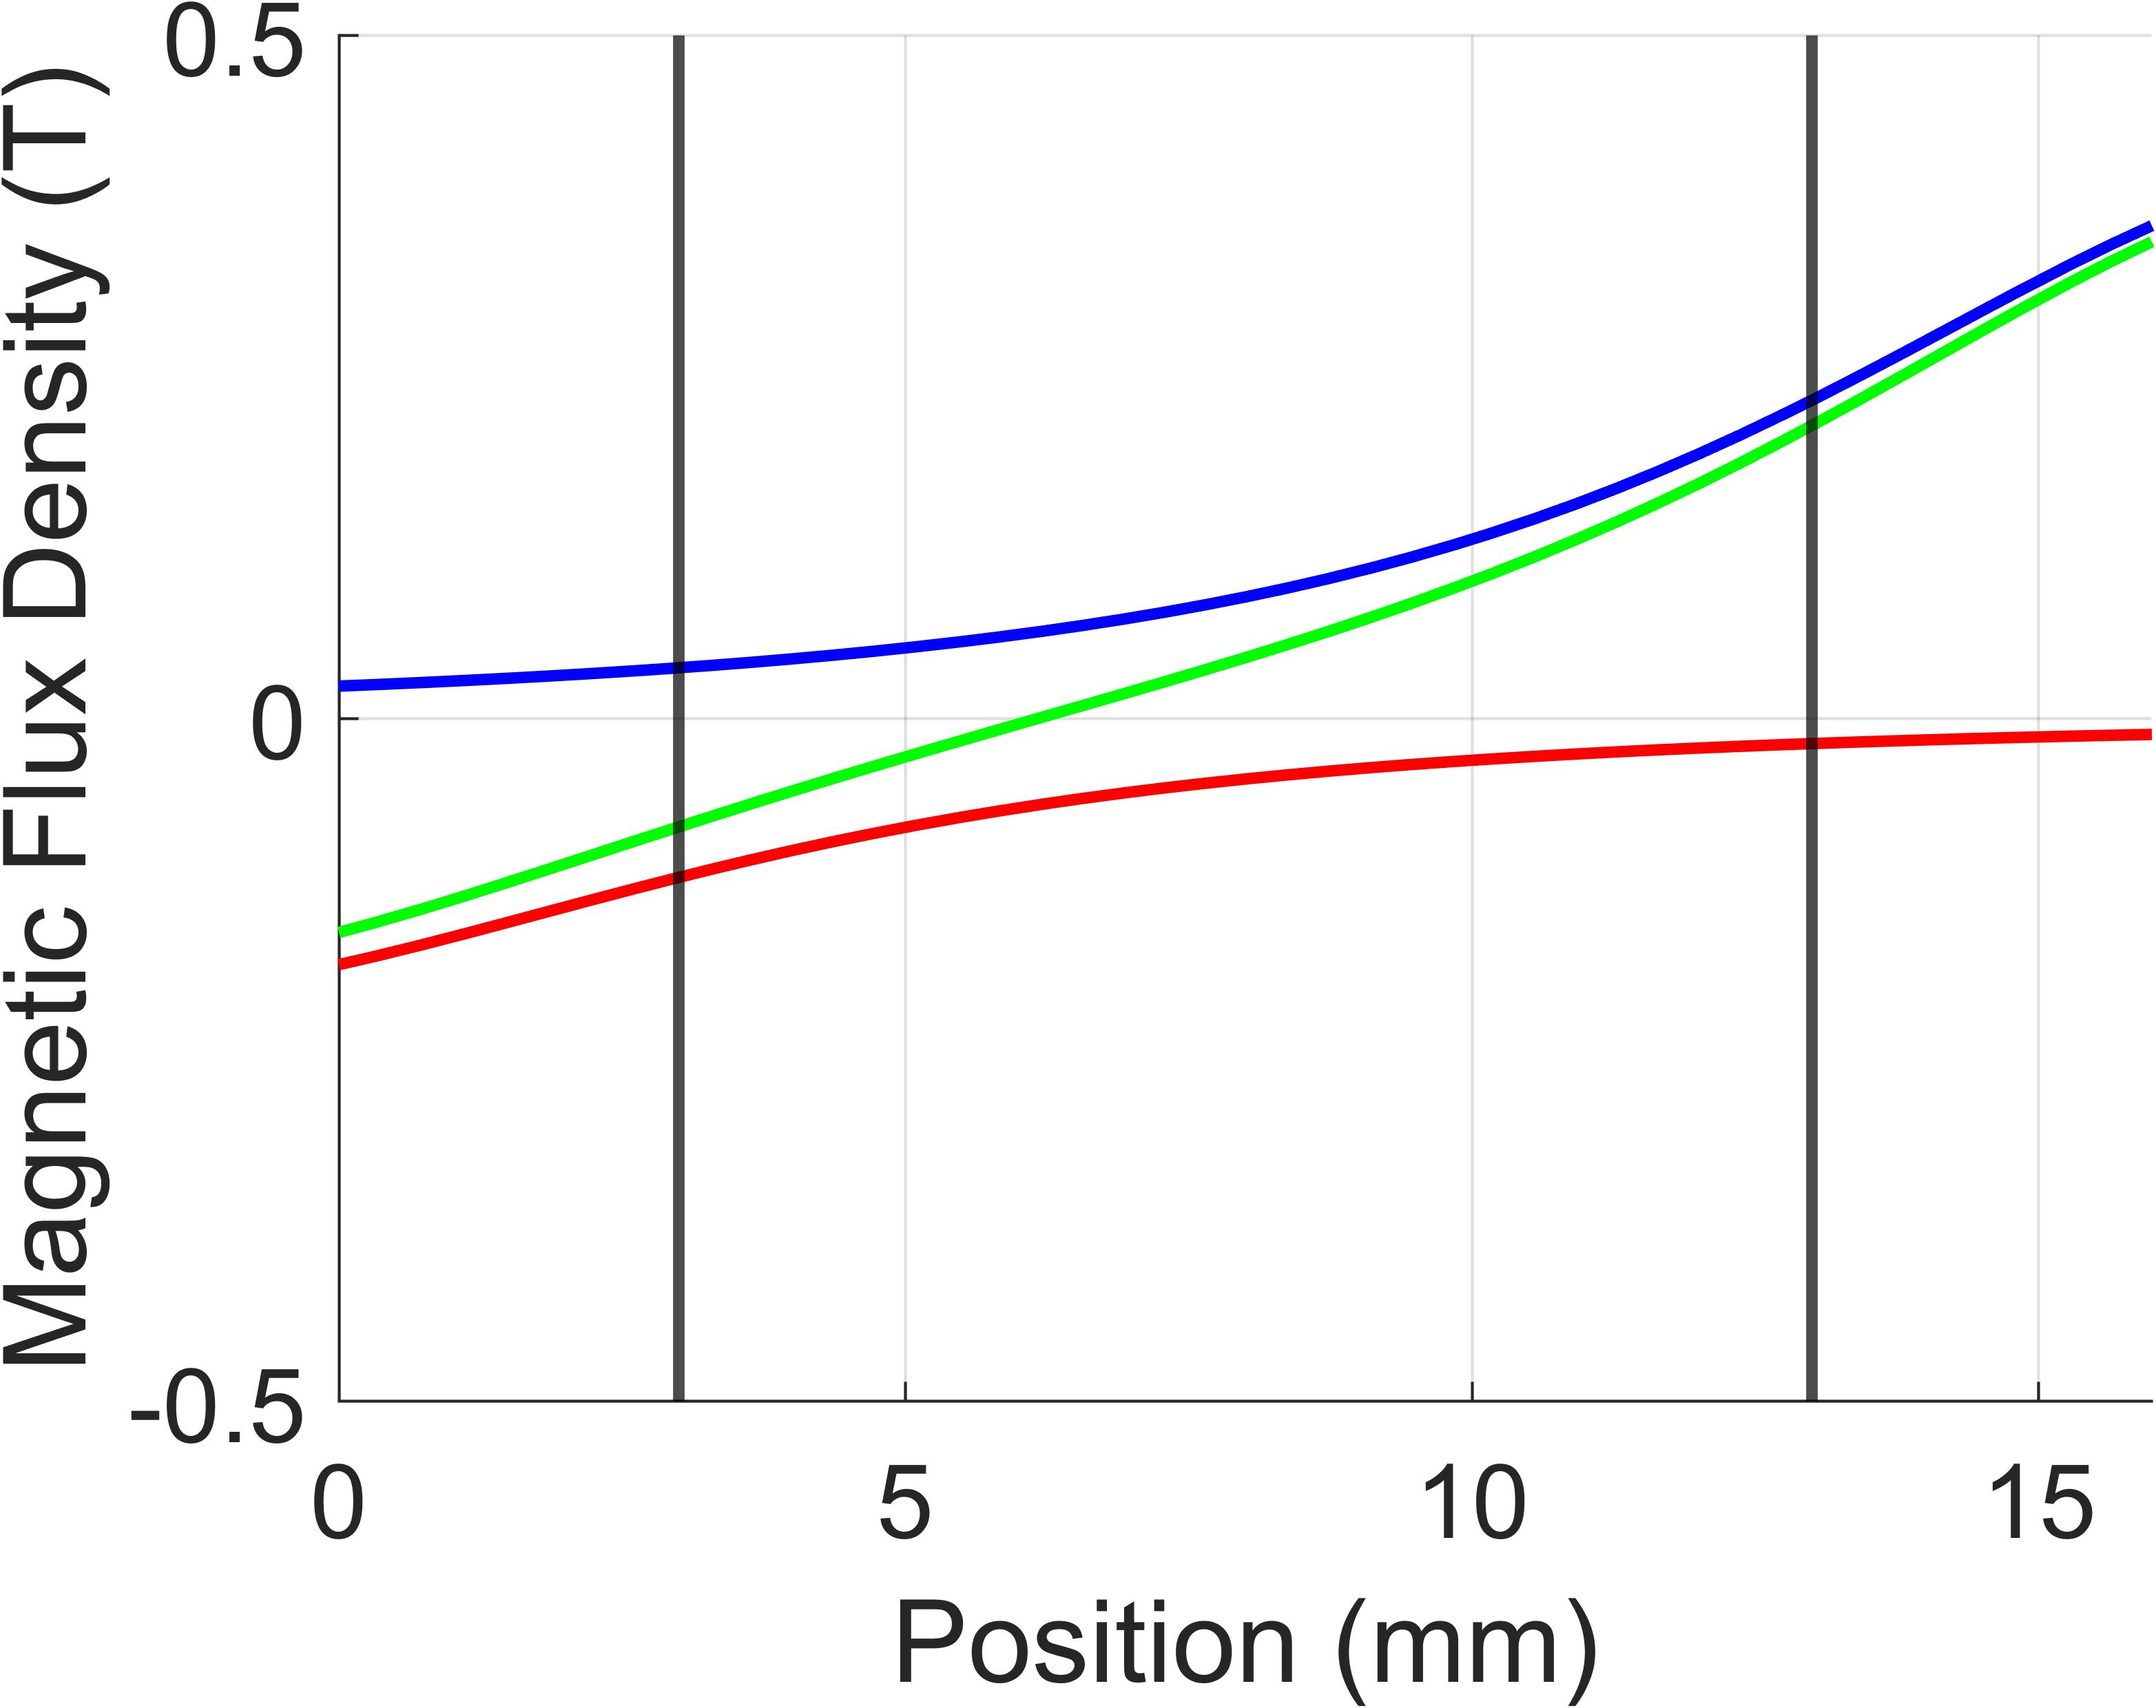
\includegraphics[width=.9\linewidth]{FluxOneTwentyDeg.jpg}
		\caption{\SI{120}{\degree} Phase}
		\label{fig:Flux120}
	\end{subfigure}
	\hfill
	\begin{subfigure}[b]{.475\textwidth}
		\centering
		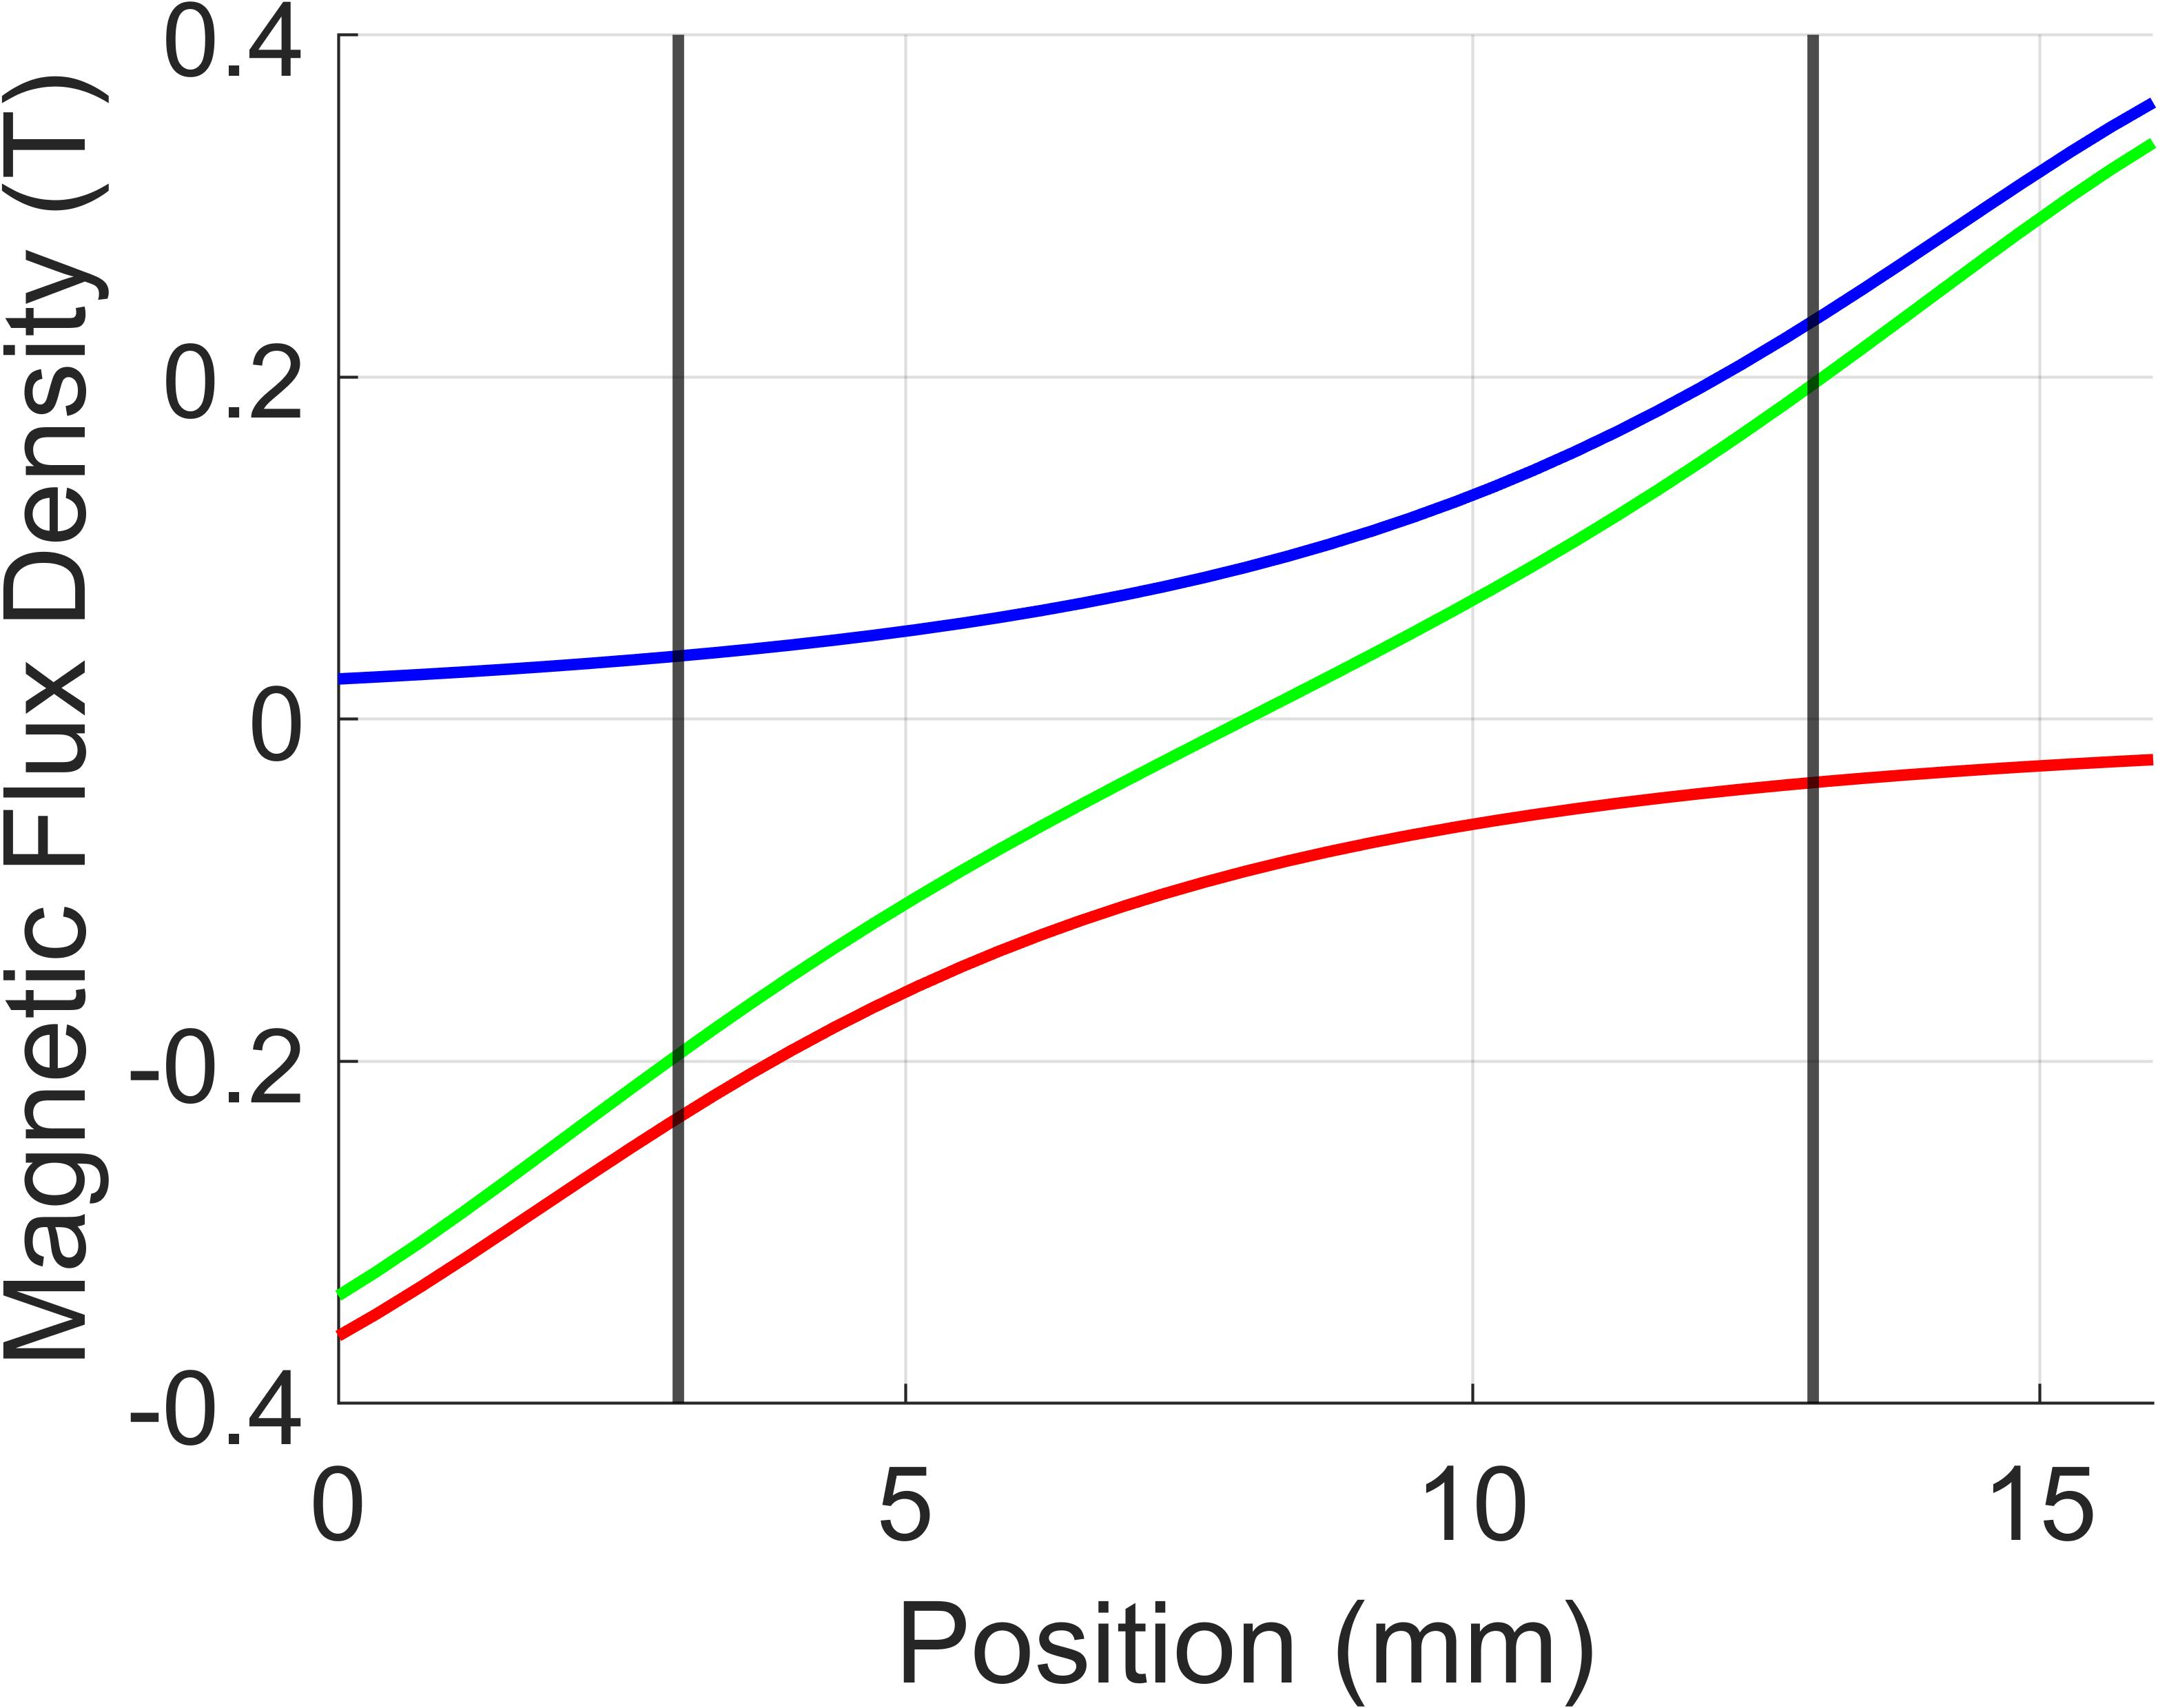
\includegraphics[width=.9\linewidth]{FluxOneEightyDeg.jpg}
		\caption{\SI{180}{\degree} Phase}
		\label{fig:Flux180}
	\end{subfigure}
	\begin{subfigure}{.475\textwidth}
		\centering
		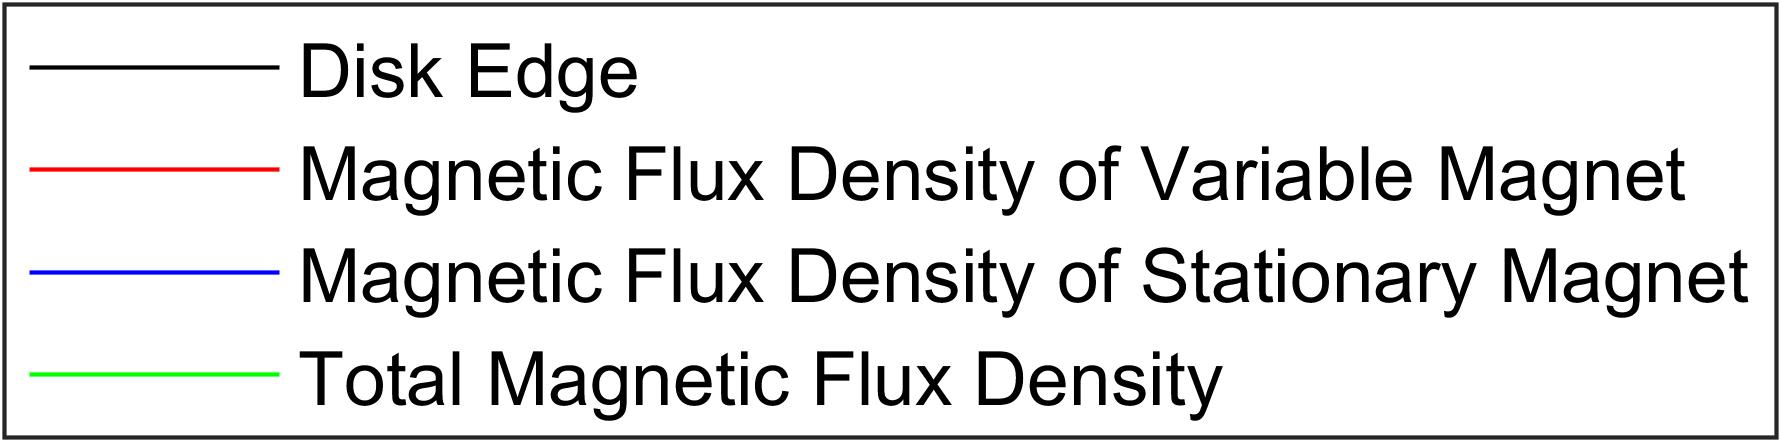
\includegraphics[width=\linewidth]{FluxLegend.jpg}
	\end{subfigure}
	\caption{Flux Distribution}
	\label{fig:Flux}
\end{figure}

\begin{figure}[h!]
	\begin{center}
		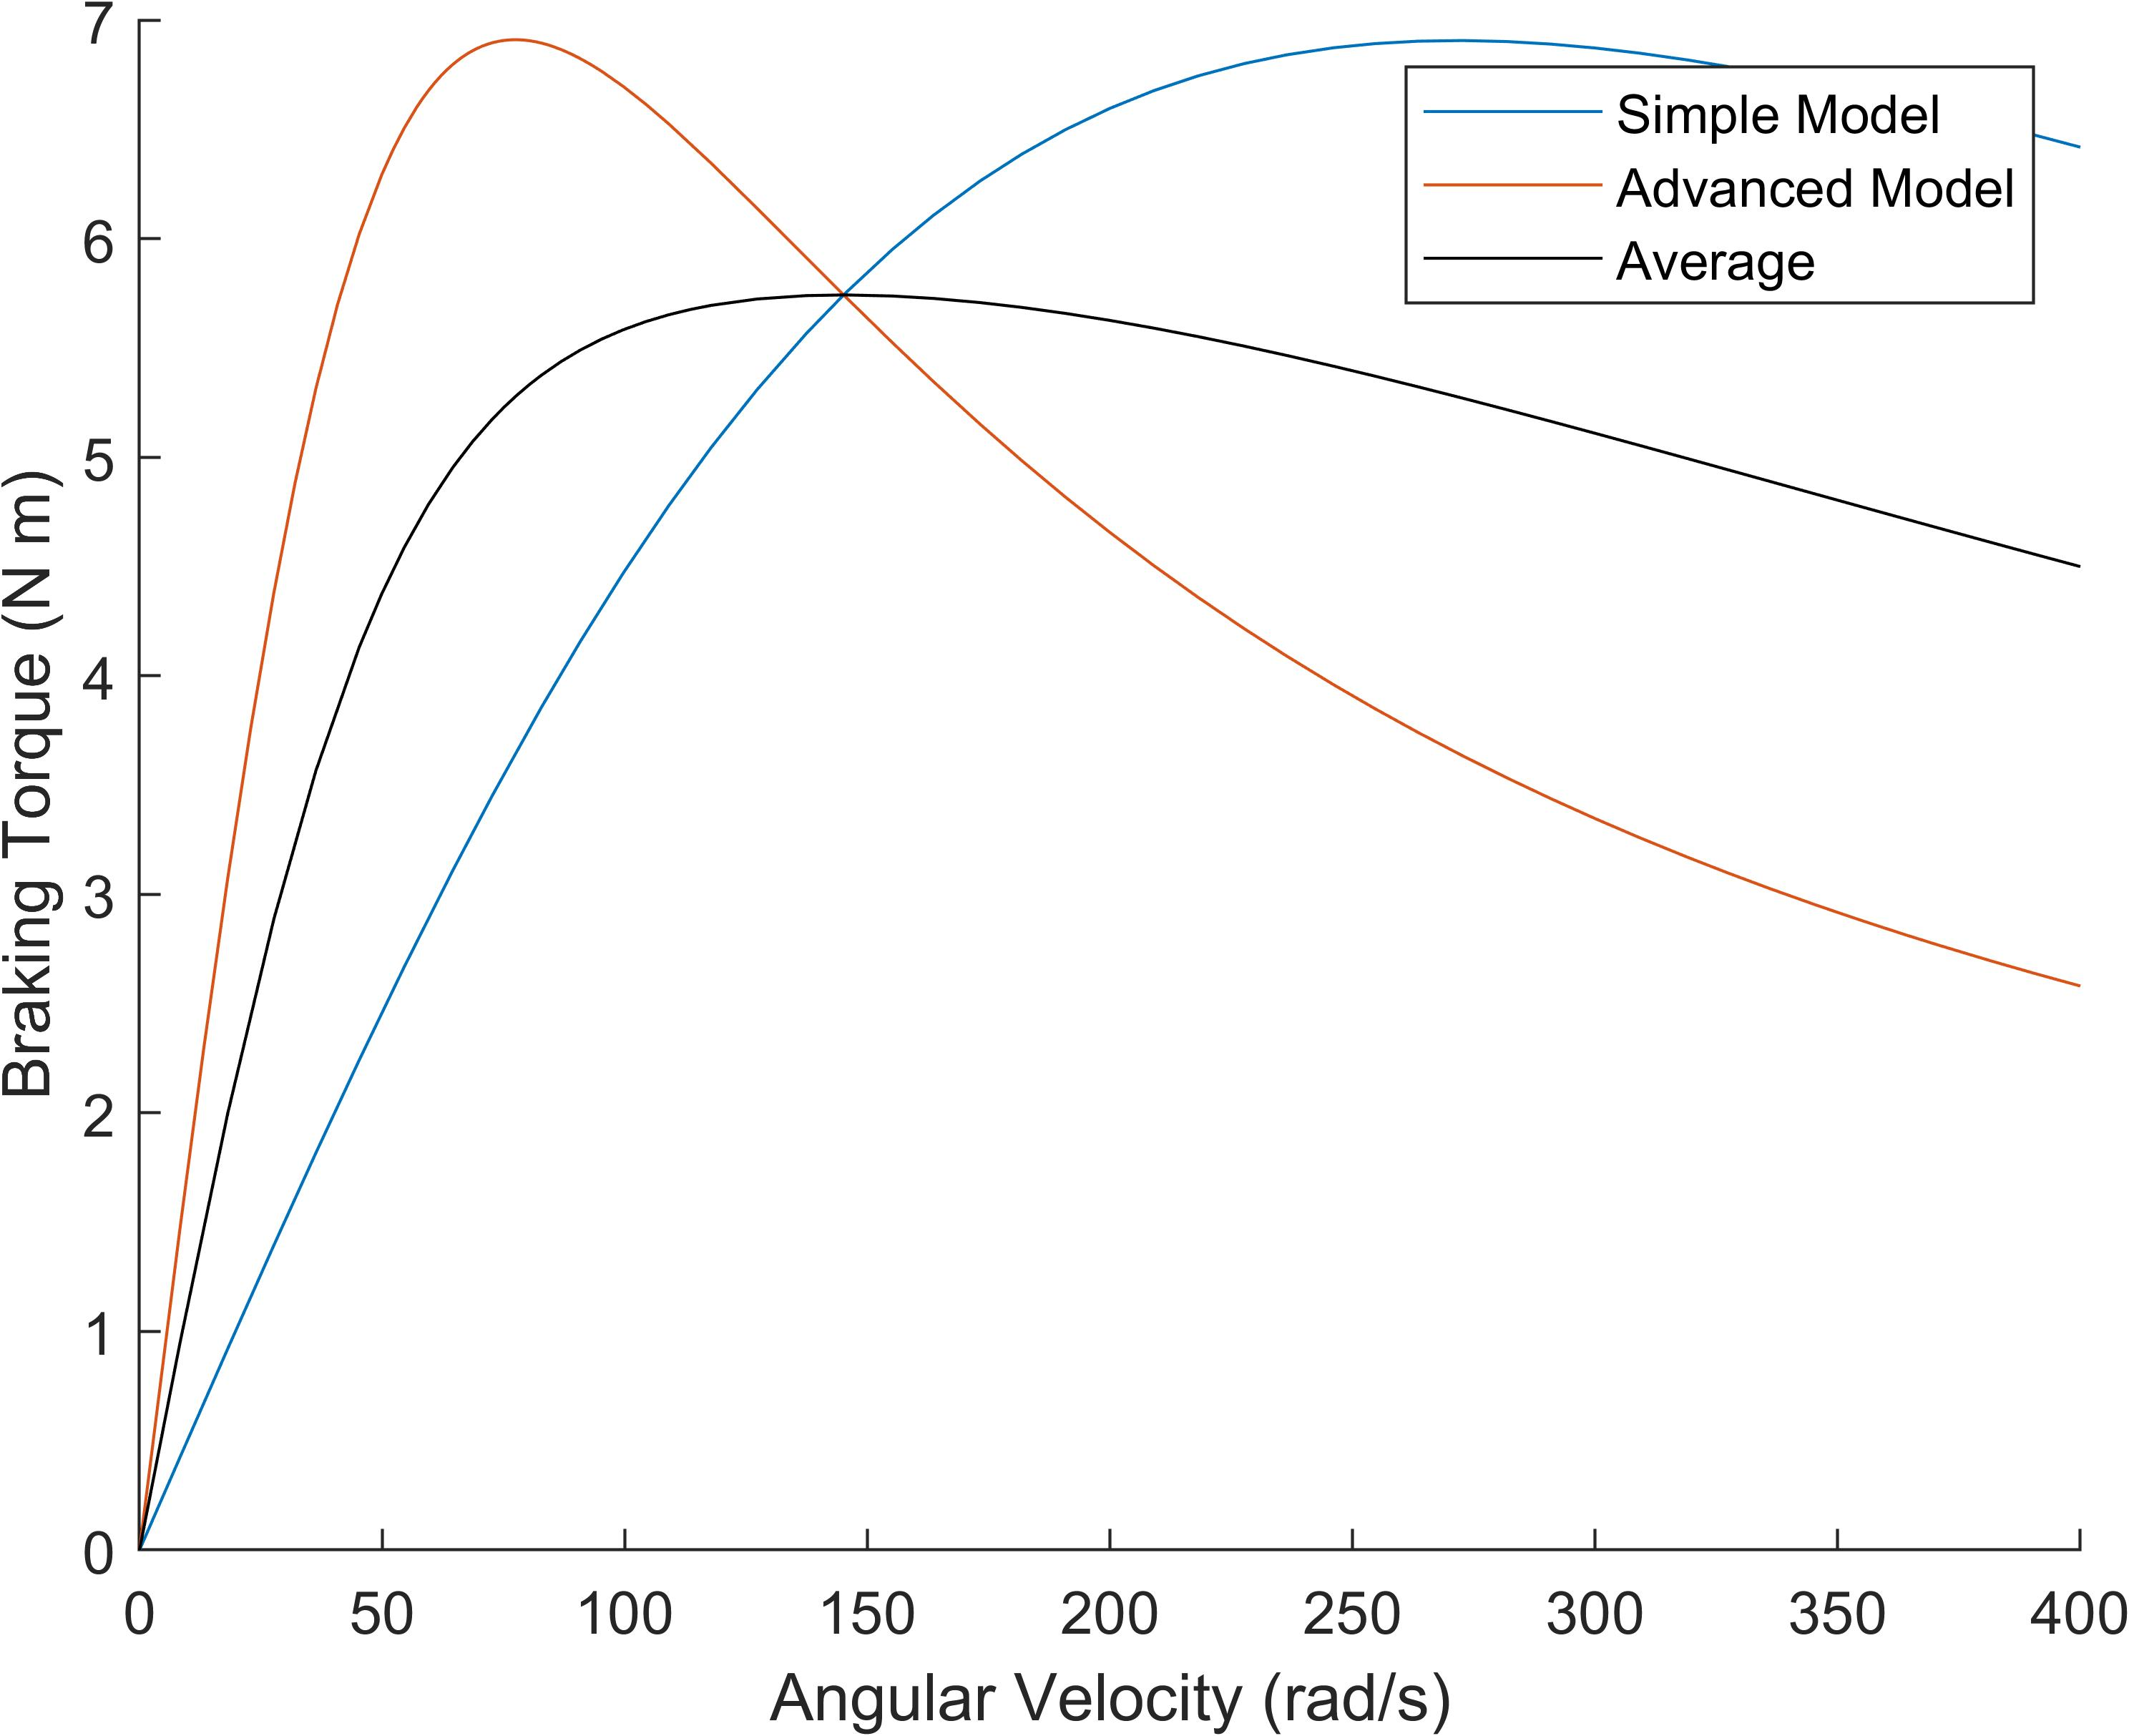
\includegraphics[width=0.8\textwidth]{Fig7.jpg}
		\caption{Figure 7}
		\label{fig:7}
	\end{center}
\end{figure}

\begin{figure}[h!]
	\begin{center}
		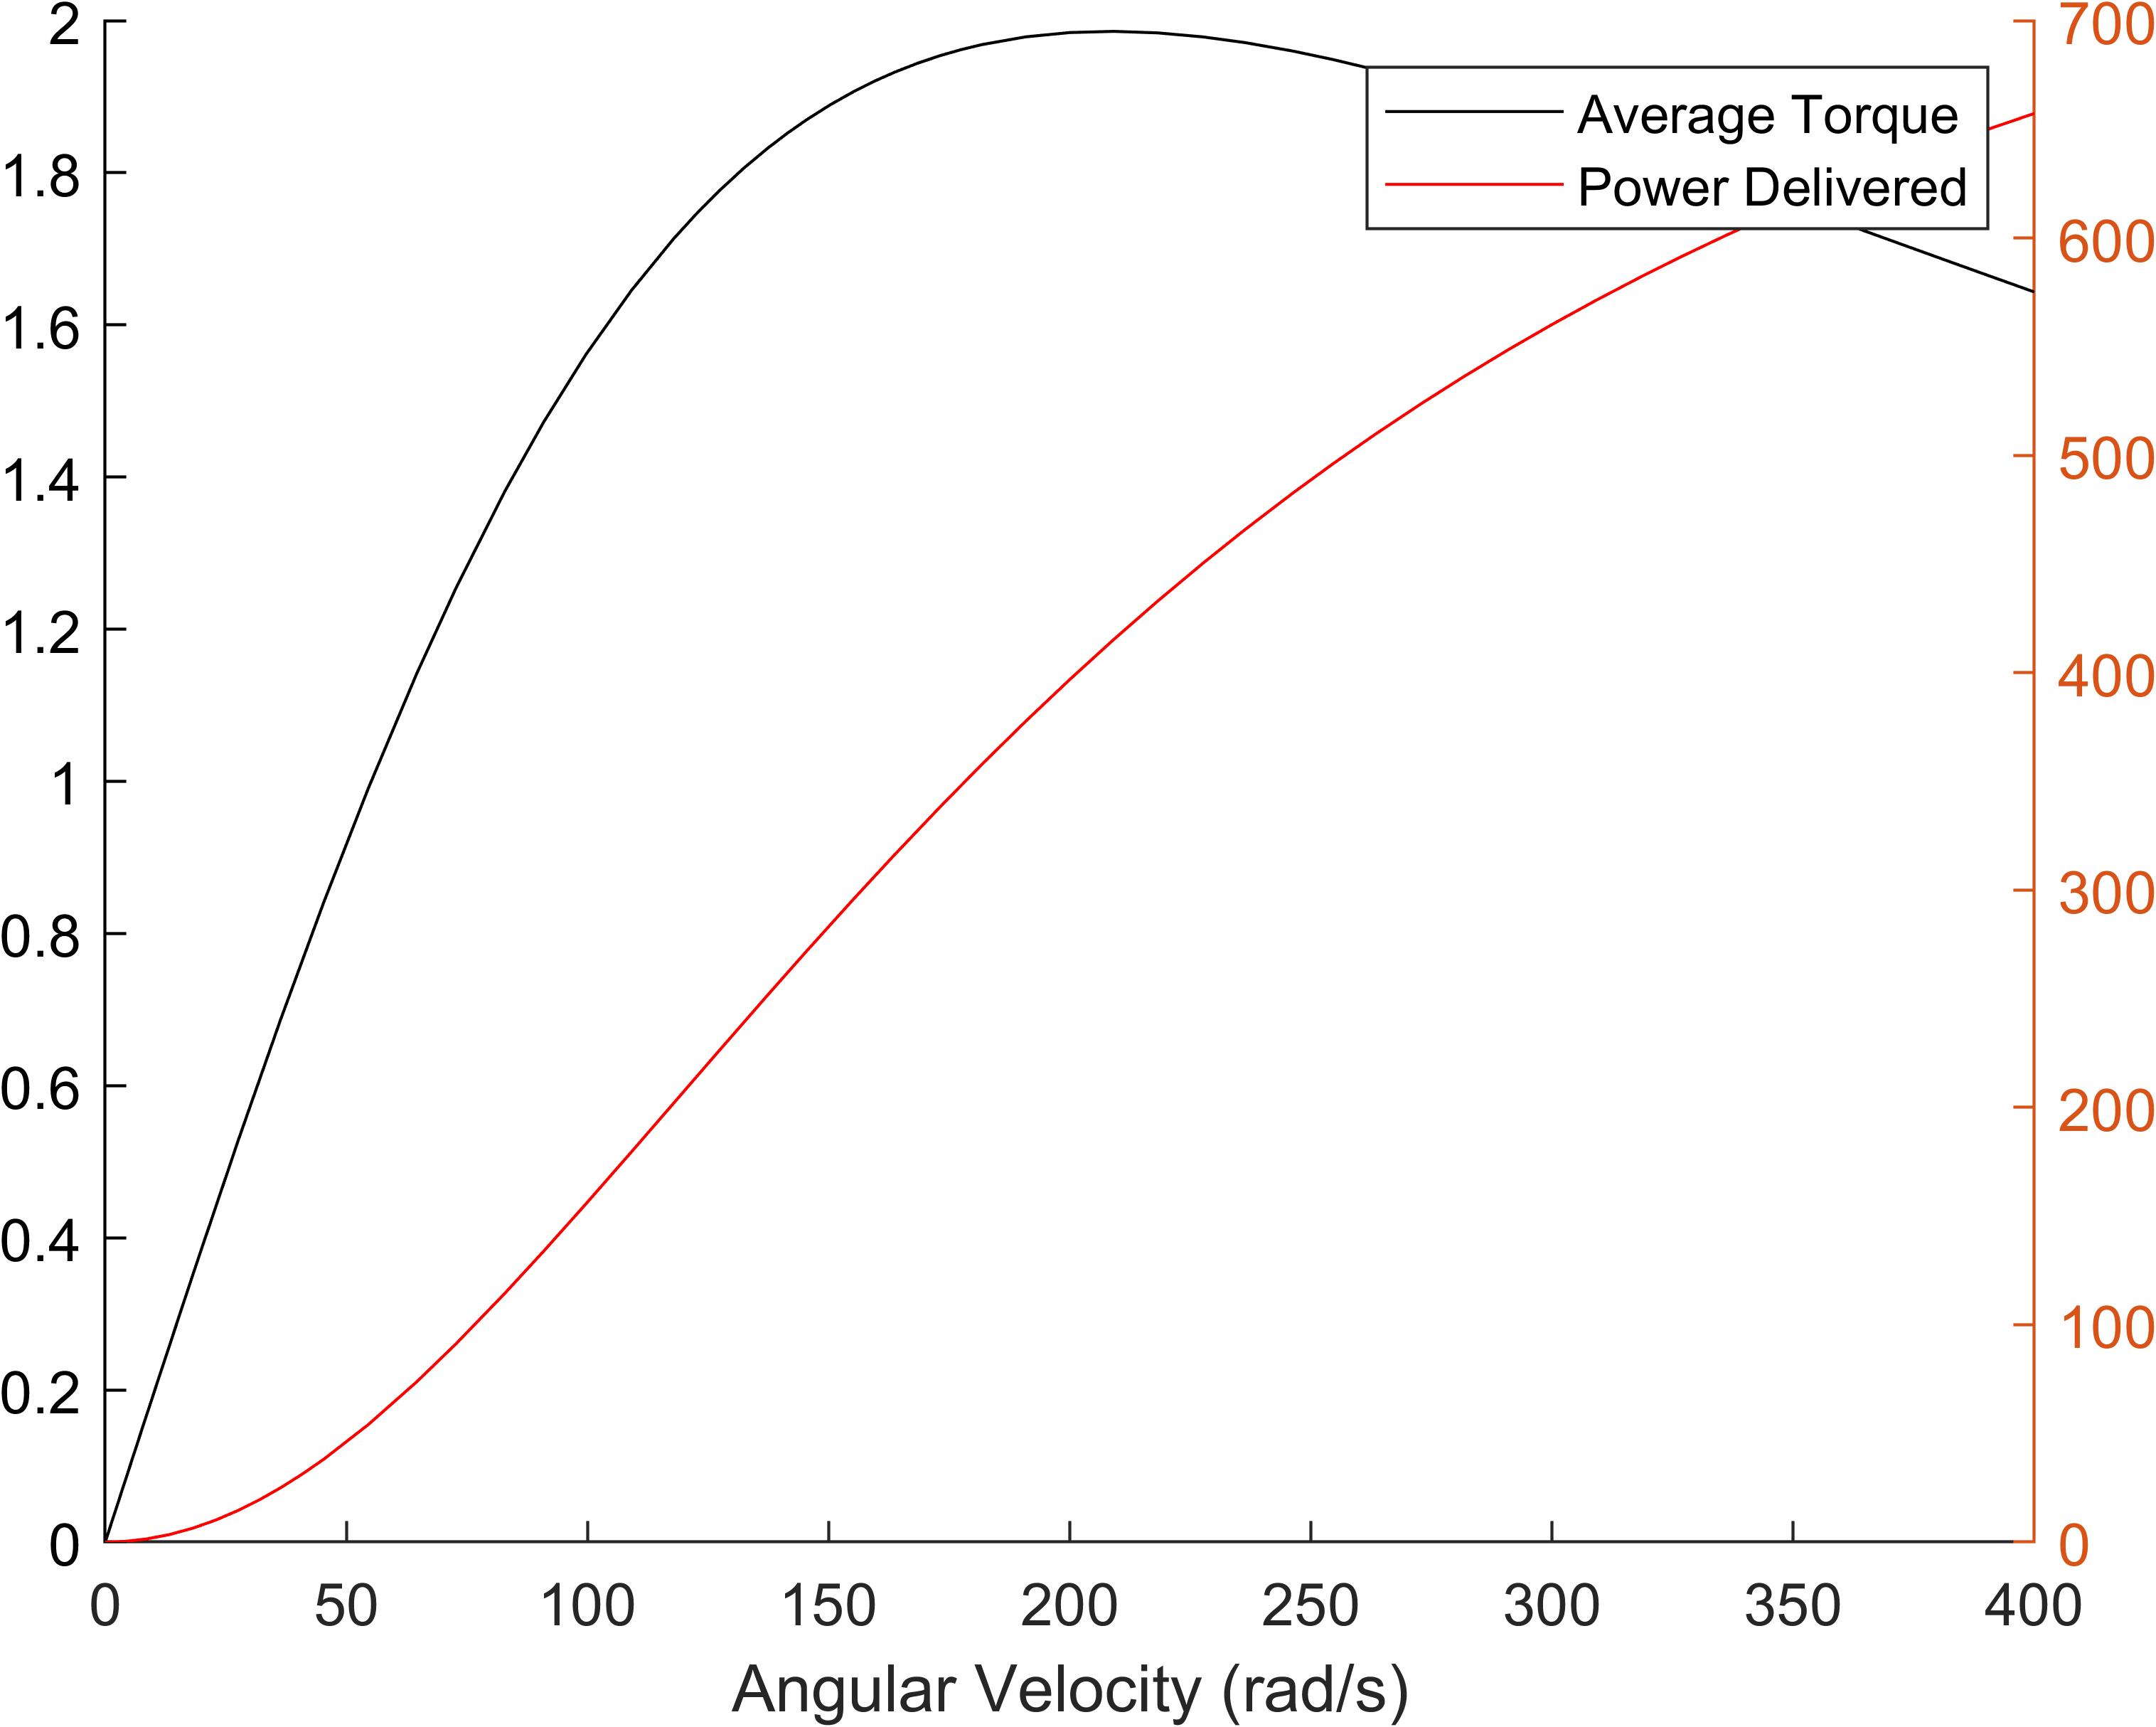
\includegraphics[width=0.8\textwidth]{Fig8.jpg}
		\caption{Figure 8}
		\label{fig:8}
	\end{center}
\end{figure}
